
Precise measurements
require accurate theoretical predictions in
order to maximise their impact in PDF fits.  Perturbative
calculations become more complex and time-consuming at higher  
orders due to the increasing number of relevant Feynman diagrams.
The direct inclusion of computationally
demanding higher-order calculations into iterative fits is thus
not possible currently since even the most advanced perturbative techniques in
combination with modern computing hardware do not lead to sufficiently
small turn-around times. However, a full repetition of the
perturbative calculation for small changes in input parameters is
not necessary at each step of the iteration.
Two methods have been developed which take advantage of this
to solve the problem: the $k$-factor technique and the
\emph{fast grids} technique. Both are available in \fitter.

%\begin{description}
%\item{\bf$k$-factor technique:}
\subsection{$k$-factor Technique}
  The $k$-factors are defined as the ratio of the prediction of a
  higher-order (slow) pQCD calculation to a lower-order (fast)
  calculation using the same PDF. Because the $k$-factors depend on the phase space
  probed by the measurement, they have to be stored  
including their dependence on
  the relevant kinematic variables. Before the start of  
  a fitting procedure, a table of $k$-factors is computed once
  for a fixed PDF with the time consuming higher-order code. In
  subsequent iteration steps the theory prediction is derived from the
  fast lower-order calculation by multiplying the pre-tabulated
  $k$-factors.

  This procedure, however, neglects the fact that the $k$-factors are 
  PDF dependent, and 
  as a consequence, they have to be re-evaluated
  for the newly determined PDF at the end of the fit for a consistency
  check. The fit must be repeated until input and output
  $k$-factors have converged. In summary, this technique avoids
  iteration of the higher-order calculation at each step, but still
  requires typically a few iterations.

In \fitter the $k$-factor technique is also used for the fast 
computation of the time-consuming GM-VFN schemes for heavy quarks in DIS.
``FAST'' heavy-flavour schemes are implemented
with $k$-factors defined as the ratio of
calculations at the same perturbative order but for massive vs.\
massless quarks, e.g.\ NLO (massive)/NLO (massless).
These $k$-factors are calculated only for the
starting PDF and hence, the ``FAST'' heavy flavour schemes should
only be used for quick checks. Full heavy flavour schemes
should be used by default. However, for the ACOT scheme,
due to exceptionally long computation time, the $k$-factors are used in 
the default settings in \fitter. 

%\vspace*{0.25cm}
%\item{\bf{}Fast grid technique:}
\subsection{\emph{Fast Grid} Techniques}

  \emph{Fast grid} techniques exploit the fact that iterative PDF fitting
  procedures do not impose completely arbitrary changes to the types
  and shapes of the parameterised functions that represent each PDF\@.
  Instead, it can be assumed that a generic PDF can be approximated by
  a set of interpolating functions with a sufficient number of
 judiciously chosen support points. The 
  accuracy of this approximation is checked and optimised 
 such that the approximation bias is negligibly
  small compared to the experimental and theoretical accuracy. 
   This method can be used to perform
  the time consuming higher-order calculations (Eq.~\ref{eq:fact})
  only once for the set of interpolating functions. 
  Further iterations of the calculation for
  a particular PDF set are fast, involving only sums over
  the set of interpolators multiplied by factors depending on the
  PDF\@. This approach can be used to calculate the cross sections 
  of processes involving one or two hadrons in the initial state and to
  assess their renormalisation and factorisation scale variation.

  This technique was pioneered by the \fastnlo
  project~\cite{Kluge:2006xs} to facilitate the inclusion of
   time consuming NLO jet cross section predictions into PDF fits.
  The \applgrid~\cite{Carli:2010rw} project developed an alternative method
  and, in addition to jets, extended its applicability to other scattering processes, 
  such as DY and heavy quark pair production is association with boson production.
  The packages differ in their interpolation
  and optimisation strategies, but both packages construct tables with
  grids for each bin of an observable in two steps: in the first step,
  the accessible phase space in the parton momentum fractions $x$ and
  the renormalisation and factorisation scales \mur and \muf is
  explored in order to optimise the table size. In the second step
  the grid is filled for the
  requested observables. Higher-order cross sections can then be
  obatined very efficiently from the pre-produced grids while varying
  externally provided PDF sets, \mur and \muf, or the strong coupling
  $\alpha_s(\mu_R)$. This approach can in principle be extended to arbitrary
  processes. This requires an interface between the
  higher-order theory programs and the fast interpolation
  frameworks. Currently available processes for each package are as follows:

\begin{itemize}
  \item The \fastnlo project~\cite{Kluge:2006xs} has been interfaced
    to the \nlojetpp program~\cite{Nagy:1998bb} for the calculation of
    jet production in DIS~\cite{Nagy:2001xb} as well as 2- and 3-jet
    production in hadron-hadron collisions at
    NLO~\cite{Nagy:2003tz,Nagy:2001fj}.  Threshold corrections at 2-loop
    order, which approximate the NNLO for the inclusive jet cross
    section, have also been included into the framework \cite{Wobisch:2011ij} 
    following Ref.~\cite{Kidonakis:2000gi}.
  
    The latest version of the \fastnlo convolution program~\cite{Britzger:2012bs} allows for the
    creation of tables in which renormalisation and factorisation scales
    can be varied as a function of two pre-defined observables, e.g.\ jet
    transverse momentum \pperp and $Q$ for DIS\@. 
    The \fastnlo code is available online \cite{fastNLO:HepForge}.
    Jet cross-section grids computed for the kinematics of various experiments
    can be downloaded from this site.

    Dedicated \fastnlo libraries and tables with theory predictions  for comparison to
    particular cross section measurements are included into the \fitter package. 
    For the \fitter implementation, the evaluation of the strong coupling constant is done
    consistently with the PDF evolution from the \qcdnum code. 

\item In the \applgrid package~\cite{Carli:2010rw,APPLGRID:HepForge},
    in addition to jet cross sections for
    $pp(\bar p)$ and DIS processes, calculations 
    of DY production are also implemented. The grids are generated with
    the customised versions of the \mcfm parton level DY
    generator~\cite{Campbell:1999ah,Campbell:2000je,Campbell:2010ff}.
    Variation of the renormalisation and factorisation scales is possible a posteriori,
    when calculating theory predictions with the \applgrid  tables, and
    independent variation of the strong coupling constant is also allowed.
    For NNLO predictions in \fitter, the $k$-factors technique can be also applied
    within the \applgrid framework.

    As an example, the \fitter interface to \applgrid was used by the ATLAS
    collaboration to extract the strange quark density of the proton
    from $W$ and $Z$ cross sections~\cite{atlas:strange}. The 
   ATLAS strange PDF extracted employing these techniques
    is displayed in
    Fig.~\ref{fig:atlas} together with a comparison to the global PDF
    sets CT10~\cite{CT10pdf} and NNPDF2.1 \cite{NNPDFpdf} (taken from \cite{atlas:strange}).

\begin{figure}[!ht]
  \centering
  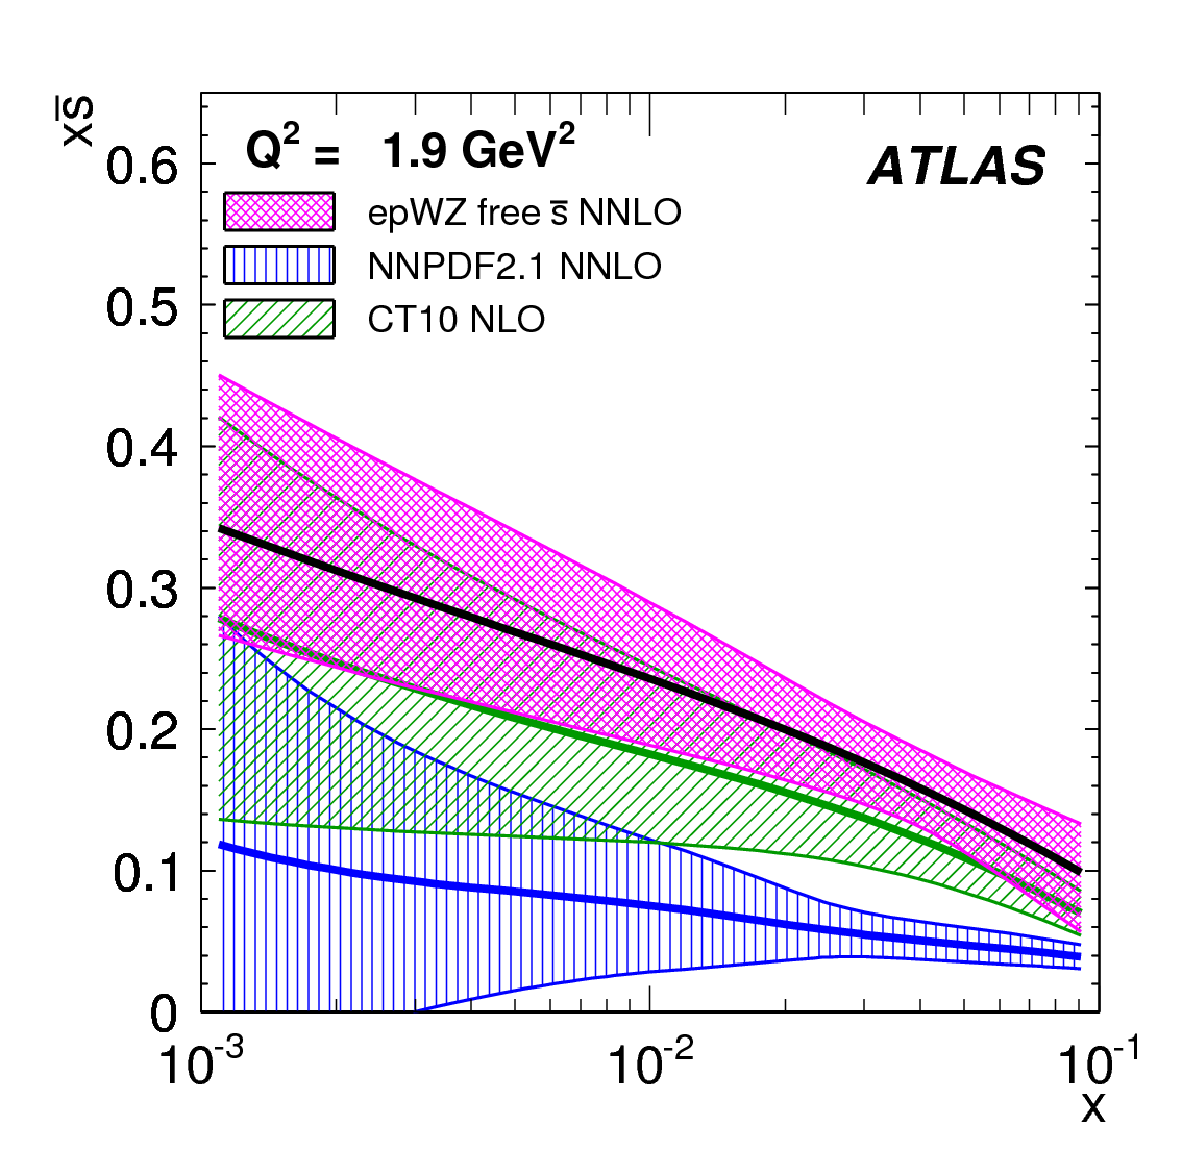
\includegraphics[width=8cm]{atlas.pdf}
  \caption{The strange antiquark density versus $x$ for the ATLAS
    epWZ free sbar NNLO fit \cite{atlas:strange} (magenta band) compared to predictions
    from NNPDF2.1 (blue hatched) and CT10 (green hatched) 
    at $Q^2 = 1.9\ \GeV^2$. The ATLAS fit was performed using a $k$-factor approach 
    for NNLO corrections.}
  \label{fig:atlas}
\end{figure}

\end{itemize}


